We first tested the accuracy of \osprey 3.0 for the subset of algorithms also available in \osprey 2.2$\beta$, by running both versions of \osprey on the same test cases and checking that the results matched.  Since the accuracy of \osprey 2.2$\beta$ using these algorithms has been experimentally confirmed (see Introduction), by transitivity, our tests confirmed \osprey 3.0's accuracy.  In addition, we performed new, retrospective tests, described below.    

To evaluate the accuracy of the implementation of the newest optimizations in \osprey 3.0, we performed a series of designs for a variety of protein-protein interfaces (PPIs) as retrospective validation. We used \ks \cite{K*} to computationally predict experimentally measured changes in binding for each PPI. Each protein structure is listed by name and PDB ID in Table \ref{table:spearman} \cite{pdb1x1u,pdb2pcb,pdb3s9d,pdb2b5i}.  These systems include barnase with its peptide inhibitor barstar \cite{binding2barnase,bindingbarnase}, the cytochrome {\it c}:cytochrome {\it c} peroxidase complex \cite{bindingcytc}, interferon $\alpha$-2 (IFN$\alpha$2) in complex with interferon $\alpha/\beta$ receptor 2 (IFNAR2)\cite{bindingifna2}, and the interleukin 2 (IL-2):IL-2 receptor $\alpha$ (IL-2R$\alpha$) complex \cite{bindingil2}.

Our retrospective validation experiments focused on mutations at residues in or proximal to the protein-protein interface that were not limited to alanine scanning. Including some of these tested and reported mutations \cite{binding2barnase,bindingbarnase,bindingcytc,bindingifna2,bindingil2}, for each structure we tested anywhere from 5 to 19 designs. In total, we tested 58 mutations using default, out-of-the-box \osprey 3.0 settings and parameters. Each design included one or two mutable residues along with a set of surrounding flexible residues (See Table \ref{table:spearman}). Flexible residues were chosen by selecting all residues within 4 {\AA} of the mutable residues and removing those that only have backbone interactions. Two example designs are shown in Figure \ref{fig:designs}, where \osprey 3.0 and \ks accurately predict the effect of two point mutations in the interface of the IFN$\alpha$2:IFNAR2 complex (highlighted in blue in Table \ref{table:spearman}). 

For each system, the \ks scores were ranked in increasing order of reported experimental binding. Spearman's $\rho$ values were subsequently calculated for each system by calculating the statistical dependence between the \ks score rankings and the experimentally measured rankings (See Table \ref{table:spearman} and Figure \ref{fig:rankings}). This is a sound measure because generally the output of a design calculation that is used to decide which mutants to make experimentally is simply the intra-system ranks of the mutants. Looking at the values in Table \ref{table:spearman}, we see a high correlation in the rankings between experimentally measured binding and binding predicted by \osprey 3.0 and \ks for each system with values ranging from 0.500 to 0.795. We found that, across the tested systems, the Spearman's $\rho$ value is 0.762. This value is the Pearson correlation of the intra-system ranks of all the mutants.  Overall, these correlations are very good for design for affinity in computational protein design.      



\begin{figure}
 \center
 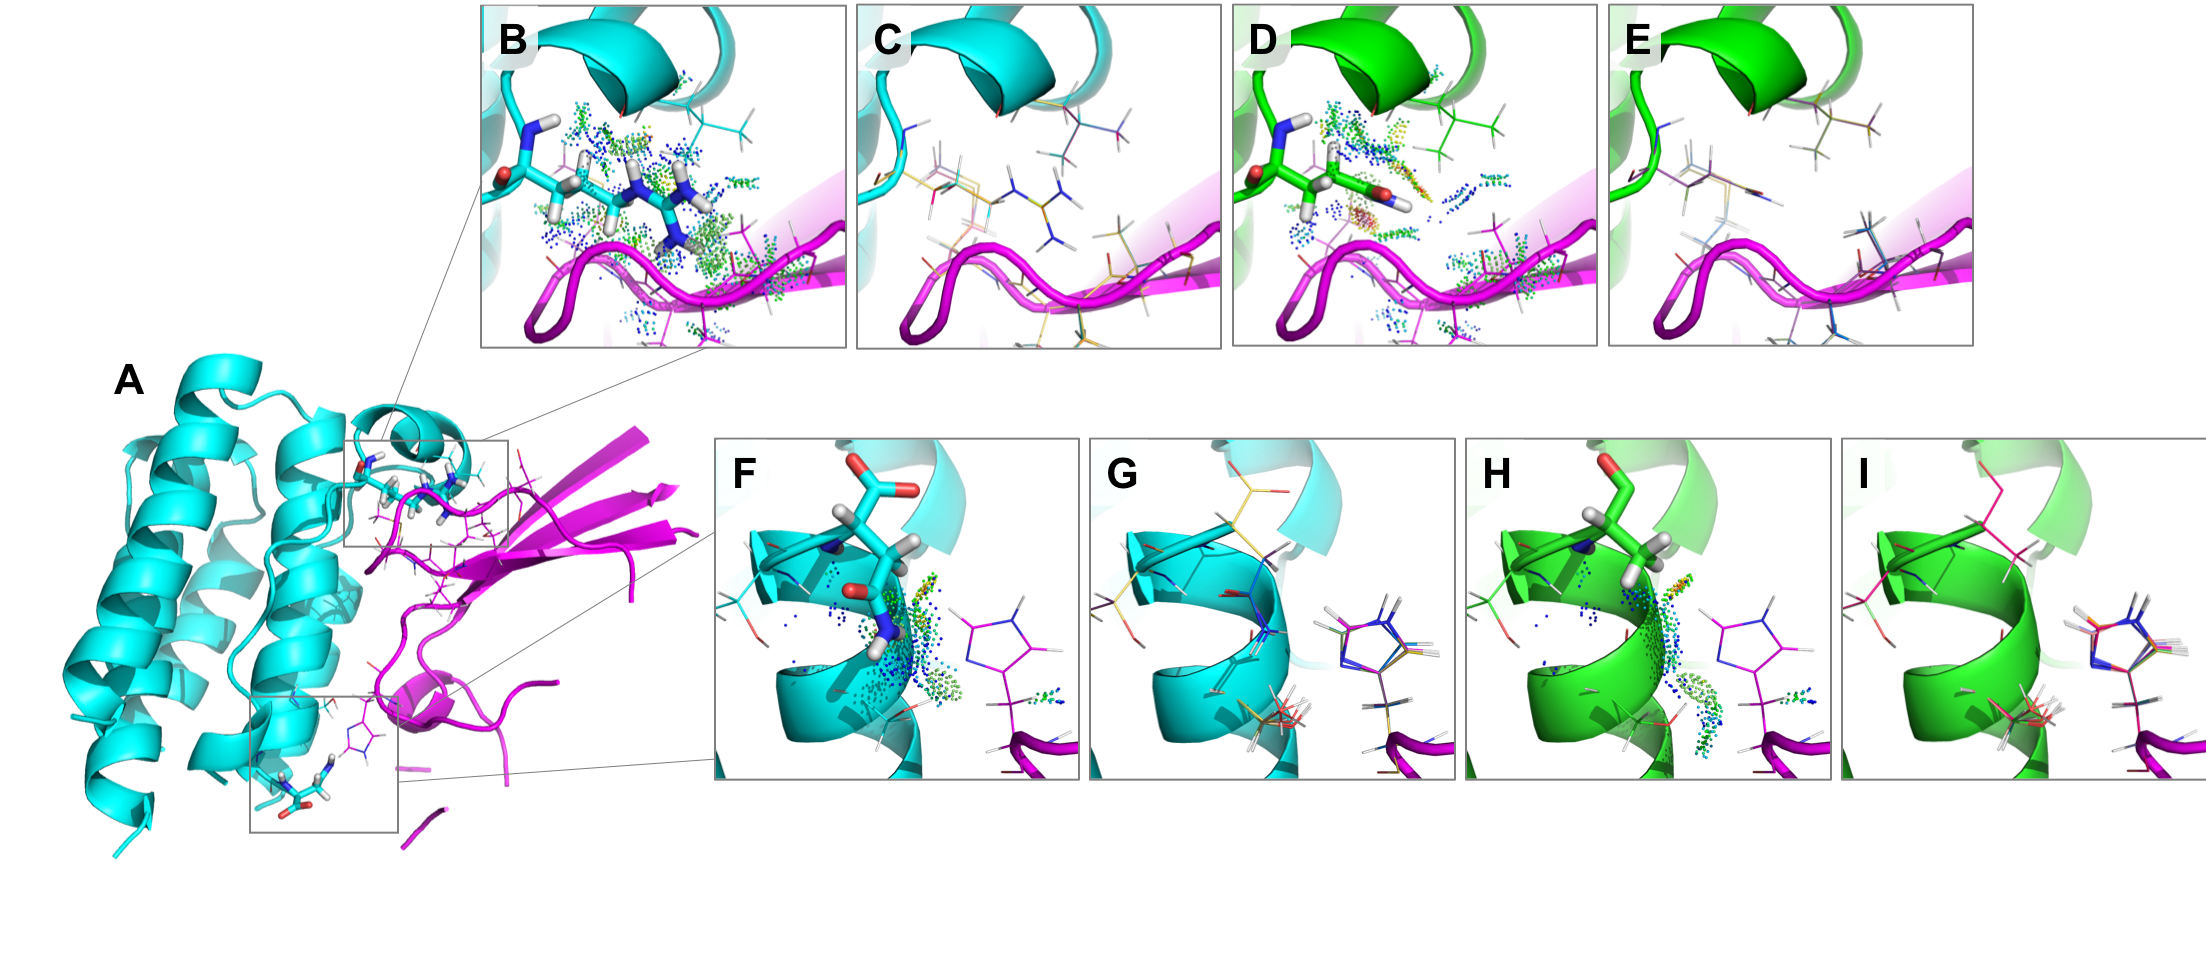
\includegraphics[width=\textwidth]{figures/designExamples.png}
 \vspace{-0.5in}%to fit the figure on one page
 \caption{(A) The structure of the IFN$\alpha$2:IFNAR2 complex (PDB ID: 3S9D \cite{pdb3s9d}) with separate chains shown in cyan and magenta and with two example interface design regions shown in boxes. Each box contains a mutable residue shown as sticks and its surrounding flexible residues shown as lines. (B) and (F) zoom in on each design. (B-E) Design at position R33 for a mutation that \osprey correctly predicts as decreasing binding: R33Q. (B) The wildtype sequence with probe dots \cite{Probe,PIV} displaying favorable interactions with surrounding flexible residues (shown as lines). (D) The mutant sequence (33Q) with probe dots displaying some favorable as well as unfavorable interactions. Comparing (B) and (D), it is clear there is a loss in favorable interactions and a gain in unfavorable interactions upon mutation from R to Q, resulting in an experimentally observed decrease in binding that the \ks algorithm captures accurately (See Table \ref{table:spearman}). (C) and (E) show the top 10 conformations in the conformational ensemble used in the \ks calculation for each sequence. (F-I) Design at position N156 for a mutation that \osprey correctly predicts as increasing binding: N156A. (F) The wildtype sequence with probe dots~\cite{Probe,PIV} displaying some favorable interactions with surrounding flexible residues (shown as lines). (H) The mutant sequence (156A) with probe dots displaying some favorable interactions with surrounding flexible residues (shown as lines). There are some gained interactions (shown by an increase in the number of favorable probe dots) in (H) compared to (F), but these are not visually obvious, thus emphasizing the importance of \ks, which successfully picks up these nuanced changes and correctly predicts improved binding (See Table \ref{table:spearman}). (G) and (I) show the top 10 conformations in the conformational ensemble used in the \ks calculation for each sequence. Not shown are the ensembles for the unbound states that are also used to calculate the \ks scores.}
\label{fig:designs}
\end{figure}

\begin{table}[h]
\centering
\scriptsize
\resizebox{.49\linewidth}{!}{
\begin{tabular}{|K{1.3cm}|K{1.7cm}|K{2cm}|K{2cm}|}
\hline
 & Mutation(s) & Experimental Ranking & Computational Ranking\\
\hline
\parbox[t]{2mm}{\multirow{13}{*}{\rotatebox[origin=c]{90}{Barnase:Barstar, PDB ID: 1X1U}}} & D39A & 1 & 1\\
 & H102A & 2 & 3\\
 & R87A & 3 & 5\\
 & K27A & 4 & 8\\
 & R59A & 5 & 2\\
 & D35A & 6 & 4\\
 & Y29A & 7 & 7\\
 & E73A & 8 & 12\\
 & E76A & 9 & 6\\
 & W35F & 10 & 11\\
 & E60A & 11 & 10\\
 & Y29F & 12 & 9\\ \cline{3-4}
 && \multicolumn{2}{c|}{$\rho = 0.755$} \\
\hline
\parbox[t]{2mm}{\multirow{17}{*}{\rotatebox[origin=c]{90}{IL-2:IL-2R$\alpha$, PDB ID: 2B5I}}} & K38E, S39D & 1.5 & 1\\
 & R35T, R36S & 1.5 & 2\\
 & R35K, R36K & 3 & 4\\
 & E1K, D4K & 4 & 7\\
 & E29R & 5 & 5\\
 & L2A & 6 & 16\\
 & D4K & 7.5 & 9\\
 & S39A, S41A & 7.5 & 12\\
 & E1K & 9 & 11\\
 & H120A & 10 & 10\\
 & E29A & 11 & 6\\
 & L42S, Y43L & 12 & 3\\
 & E1Q & 13 & 14\\
 & N27A & 14 & 15\\
 & K38T & 15 & 8\\
 & D4N & 16 & 13\\ \cline{3-4} 
 && \multicolumn{2}{c|}{$\rho = 0.554$}  \\
\hline
\end{tabular}
}
\resizebox{.49\linewidth}{!}{
\begin{tabular}{|K{1.3cm}|K{1.7cm}|K{2cm}|K{2cm}|}
\hline
\multirow{6}{*}{\rotatebox[origin=c]{90}{\parbox[t]{2.5cm}{\centering Cyt{\it{c}}:Cyt{\it{c}} peroxidase, PDB ID: 2PCB}}} & E290N & 1 & 2\\
 & D34N & 2 & 4\\
 & A193F & 3 & 1\\
 & E35Q & 4 & 3\\ 
 & E32Q & 5 & 5\\ \cline{3-4}
 && \multicolumn{2}{c|}{$\rho = 0.500$} \\ 
\hline
\parbox[t]{2mm}{\multirow{20}{*}{\rotatebox[origin=c]{90}{IFN$\alpha$2:ifnar2, PDB ID: 3S9D}}} & \colorbox{LightCyan}{R33Q} & 1 & 1\\
 & R33A & 2 & 2\\
 & R33K & 3 & 5\\
 & L30A & 4 & 6\\
 & R149A & 5 & 4\\
 & L30V & 6 & 9\\
 & A148A & 7 & 10\\
 & A145G & 8 & 14\\
 & A145M & 9 & 3\\
 & L15A & 10 & 13\\
 & L153A & 11 & 12\\
 & L26A & 12 & 7\\
 & S152A & 13 & 16\\
 & F27A & 14 & 8\\
 & S25A & 15 & 18\\
 & D35A & 16 & 17\\
 & R22A & 17 & 11\\
 & M16A & 18 & 15\\
 & \colorbox{LightCyan}{N156A} & 19 & 19\\ \cline{3-4}
 && \multicolumn{2}{c|}{$\rho = 0.795$} \\
 \hline
 \multicolumn{2}{|c|}{} & {\textbf{Across All}} & $\rho = 0.762$ \\
\hline
\end{tabular}
}
\caption{\textbf{Comparison of \osprey predictions to experimental results for mutations in four protein systems.}  Allowed mutations for each system are listed along with their corresponding rankings from experimental measurements \cite{binding2barnase,bindingbarnase,bindingcytc,bindingifna2,bindingil2} vs. computational predictions by \ks from \osprey 3.0. The mutations highlighted in blue are shown in detail in Figure \ref{fig:designs}. A Spearman's $\rho$ value is calculated for each system and shown here. The ``Across All" value is calculated by ranking each system individually and then calculating the Spearman's $\rho$ across all of the designs.}
\label{table:spearman}
\end{table}

\begin{figure}
\center
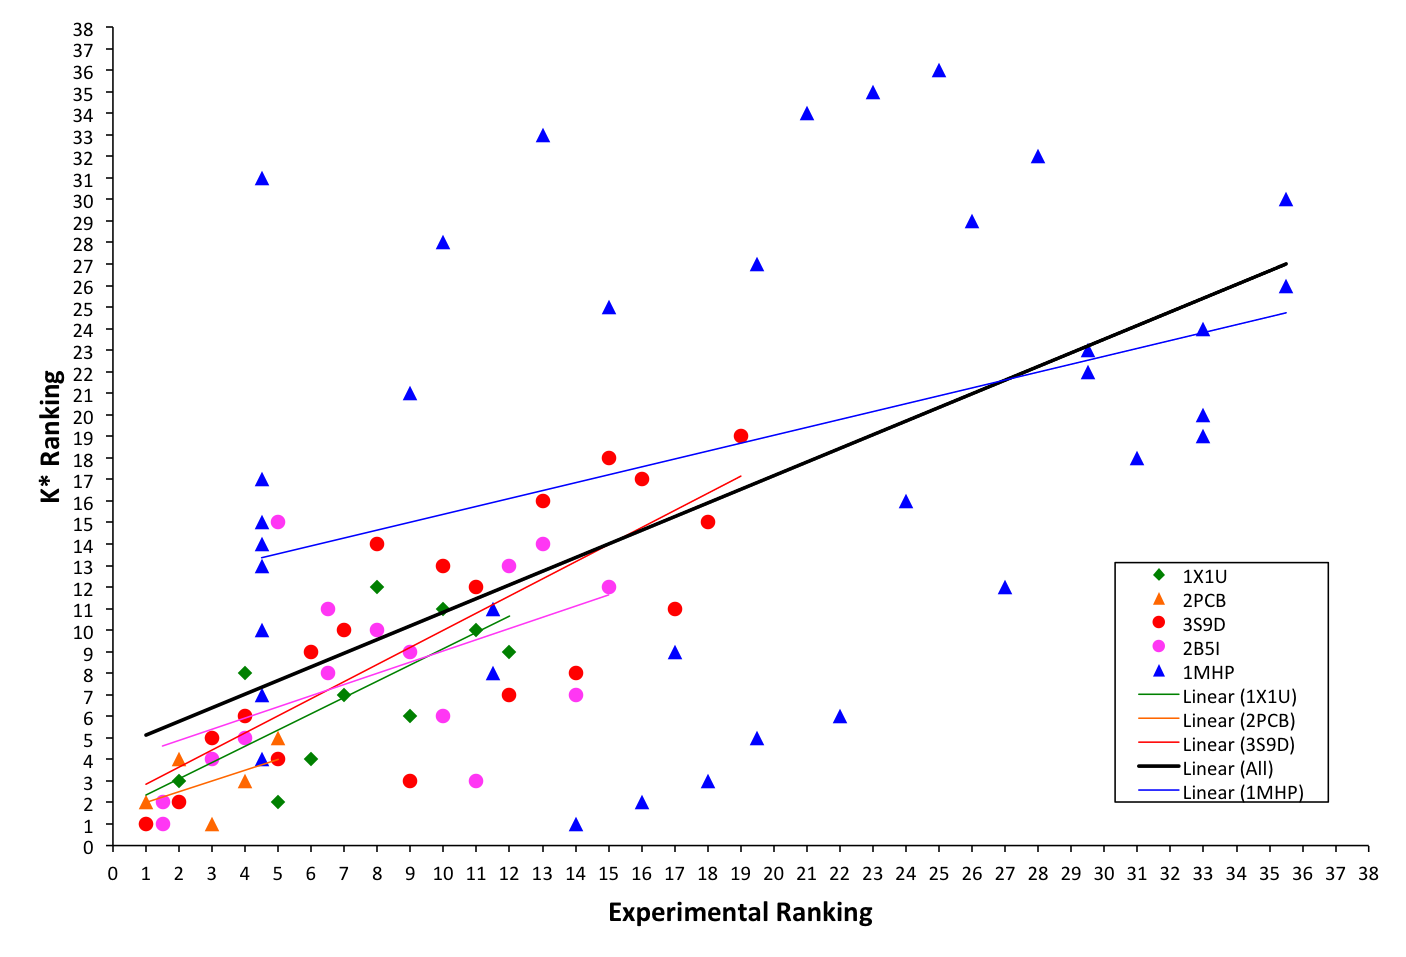
\includegraphics[width=0.9\textwidth]{figures/Rankings.png}
\caption{Testing the accuracy of the \ks algorithm in \osprey 3.0 by comparing \ks rankings to experimentally reported rankings (See Table \ref{table:spearman}). Each system is represented by its corresponding PDB ID and a linear trendline is shown for each in its corresponding color according to the legend.}
\label{fig:rankings}
\end{figure}

% \begin{table}[h!]\label{table:spearman}
% \centering
% \begin{tabular}{ |c||c|  }
%  \hline
%  \textbf{Structures (PDB ID)}& \textbf{Spearman's $\rho$} \\
%  \hline 
%  3S9D   & 0.795 \\
%  \hline
%  1X1U   & 0.755 \\
%  \hline
%  2B5I   & 0.554 \\
%  \hline
%  2PCB   & 0.500 \\
%  \hline
%  \textbf{Across Structures} &   \textbf{0.762}  \\
%  \hline
% \end{tabular}
% \caption{Spearman's $\rho$ table. A Spearman's $\rho$ value is calculated for each system and shown here. The ``Across Structures" value is calculated by ranking each system individually and then calculating the Spearman's $\rho$ across all of the designs---in other words, it is the Pearson correlation of the intra-system ranks of all the mutants.  We consider this meaningful because the output of a design calculation that is used to decide on mutants to make experimentally is simply the intra-system ranks of the mutants.  }
% \end{table}
